
\chapter{Tests et optimisations}
\label{chap:tests et optimisations}

\section{Premiers Tests de performance}

\subsection{Pr\'esentation et Valgrind}

Apr\`es avoir pr\'esent\'e les outils que nous avons utilis\'es, nous allons maintenant pr\'esent\'e les premiers tests de performances effectu\'es 
avant la fin de l'optimisation.
Ces tests sont effectu\'es \`a l'aide de la fonction time pour les temps d'ex\'ecution et valgrind pour les tests de m\'emoire.
Du fait de l'utilisation du langage C nous esp\'erons avoir des temps bien inferieurs pour l'ex\'ecution de chaque programme, c'est ce que nous allons
 v\'erifier.
L'utilisation faite de la m\'emoire telle que le nombre d'allocations ou l'espace allou\'e par chaque programme ne d\'epend pas \`a priori du langage
 utilis\'e mais plut\^ot de l'algorithmie cach\'ee dans le code, c'est pourquoi il ne devrait pas y avoir beacoup d'am\`elioration de ce c\^ot\'e l\`a,
n\'eanmoins elle reste toujours un param\`etre important faisant partie des performances d'un programme.
Nous avons ici class\'es les programmes comme dans la partie 2.
Pour tests portant sur les temps d'ex\'ecution nous utiliserons la fonction time pr\'esente dans toutes les distributions GNU/Linux \'ecrite par David MacKenzie et qui permet d'\'evaluer avec plus ou moins de pr\'ecision le temps d'ex\'ecution d'un programme.
Les tests portant sur la m\'emoire seront eux effectu\'es avec l'outil valgrind, d'habitude utilis\'e pour le d\'eboguage et la chasse aux erreurs de segmentations (lecture ou \'ecriture non autoris\'ee dans la m\'emoire).
Valgrind regroupe en fait six outils de d\'eveloppement et a \'et\'e d\'evelopp\'e par un groupe de programmeurs, il n'est pas fait \`a priori pour l'utilisation quel'on en fait dans la partie suivante (lenteur d'ex\'ecution) mais fonctionne quand m\^eme bien.
 



\subsection{Calculs simples sur des nombres d\'ecimaux}

La fonction numsum n'\'etant pas encore fiinalis\'ee cette section ne fera pas figurer de tests sur ce programme.
\newline

Ici le temps d'ex\'ecution varie selon le nombre de chiffre sur lequel on fait travailler un programme, c'est ce que nous allons observer.
La fonction numaverage comprend deux options principales. Elle permet de calculer \`a la fois, la moyenne, la m\'ediane et le mode d'une s\'erie de nombre.
\newline

Voici un graphe en \'echelle logarithmique repr\'esentant le comportement des calculs de la m\'ediane et de la moyenne en fonction du nombre de 
donn\'ees. la fonction mode n'apparait pas car elle ne supporte pas bien les grands nombres de donn\'ees et il n'y avait pas assez de points pour 
faire une courbe.

\begin{figure}[h]
\begin{center}
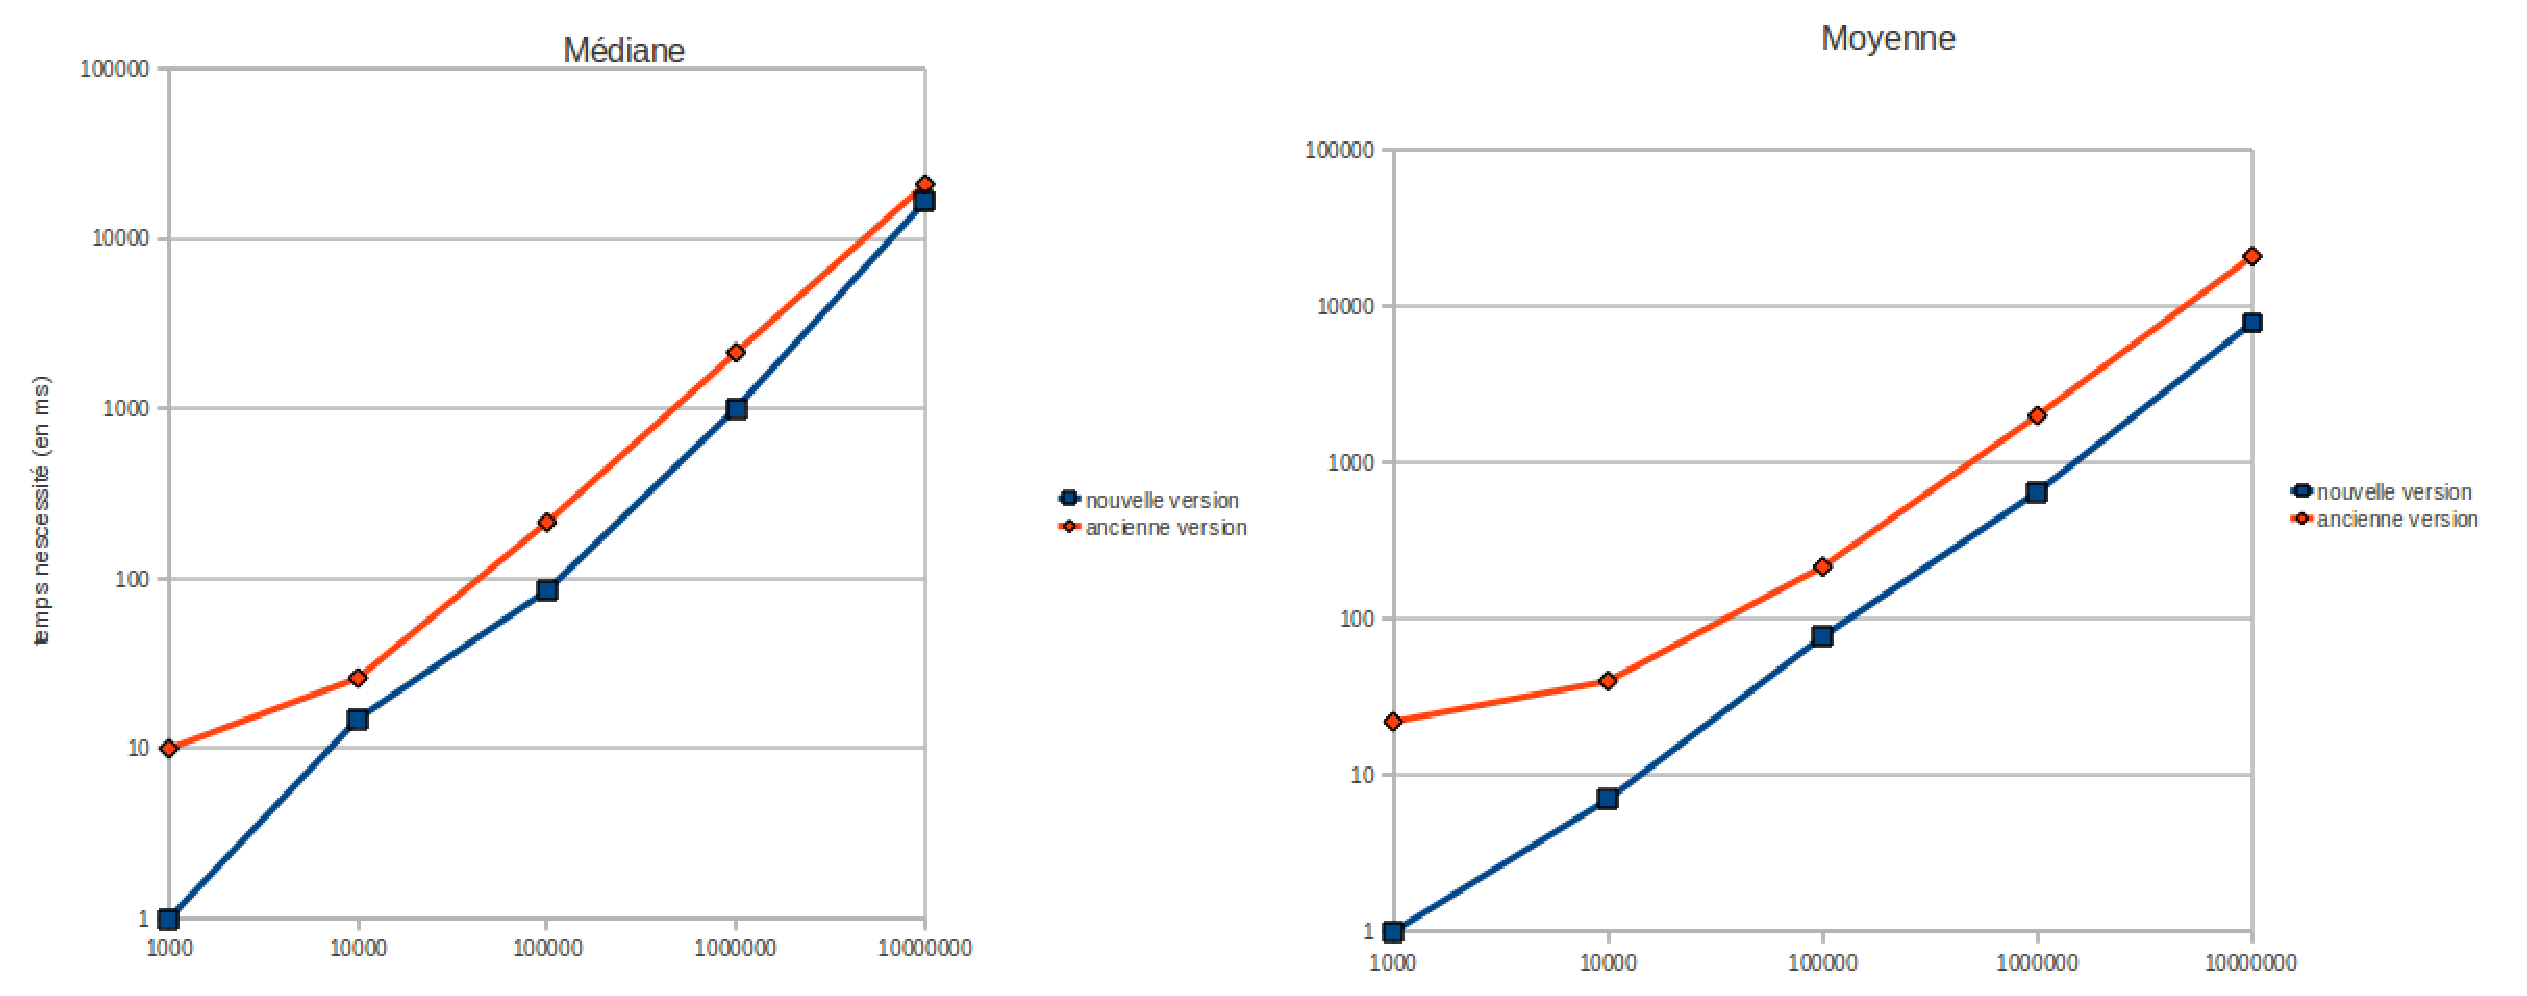
\includegraphics[width=15cm]{MoyenneMediane.eps}
\end{center}
\caption{Performances de M\'ediane et Moyenne}
\end{figure}

Et voil\`a un tableau \ref{tab:numaverage} relatant les performances de chacune de ces options (og et ng signifiant respectivement << old generation >> et << new generation >> ) : 
\newline
On voit successivement pour chaque test en premi\`ere ligne le temps d'ex\'ecution en ms, en deuxi\`eme le nombre d'allocations et enfin en troisi\`eme 
la m\'emoire allou\'ee.
\newline

\begin{table}[h]
\begin{center}
\begin{tabular}{|c|c|c|c|c|c|c|}

\hline
Nb de donn\'ees & moy (og) & moy (ng) & m\'ed (og) & m\'ed (ng) & mod (og) & mod (ng)  \\
\hline
 \multirow{3}*{1000} & 22 & 1 & 10 & 1 & 11 & 2 \\
\cline{2-7}
 & 1693 & 1 & 1693 & 1004 & 1693 & 2003 \\
\cline{2-7}
 & 183ko & 352o & 183ko & 4Mo & 183ko & 6Mo \\
\hline
 \multirow{3}*{10000} & 40 & 7 & 26 & 15 & 40 & 107 \\
\cline{2-7}
 & 1693 & 1 & 1693 & 10000 & 1693 & 2003 \\
\cline{2-7}
 & 183ko & 352o & 183ko & 400Mo & 183ko & 600Mo \\
\hline
100000 & 215 & 77 & 214 & 85 & 279 & 8024 \\
\hline
1000000 & 1991 & 647 & 2133 & 1004 &  &  \\
\hline
10000000 & 20748 & 7799 & 20802 & 16530 &  & \\
\hline
\end{tabular}
\caption{Performances de M\'ediane et Moyenne}
\end{center}
\label{tab:numaverage}
\end{table}
Remarque : Faute de temps (l'\'execution de valgrind \'etant tr\`es lente) les tests de m\'emoire n'ont pas \'et\'e fait pour de grandes s\'eries de nombre.
\newline
On peut remarquer que conform\'ement \`a nos attentes les temps d'ex\'ecution des nouveaux programmes sont bien inferieurs \`a ceux des anciens,
 n\'enamoins certains d'entre-eux ont des consommations de m\'emoire beacoup plus importantes, cela est du au fait que certains de nos programme 
ne supportent pas encore les flux de donn\'ees (en particulier la fonction qui calcule le mode), nous en reparlerons dans la partie optimisation.
Le probl\`eme de la gestion des flux de donn\'ee est un probl\`eme r\'ecurrent en algorithmie : certains programmes ont besoins d'un historique 
des donn\'ees pour faire leur calcul, ce qui devient un probl\`eme pour les grands nombres de donn\'ees.

\subsection{Comparaisons de nombres d\'ecimaux}

Dans cette partie la probl\'ematique est quasiment la m\^eme que dans la partie pr\'ec\'edente, \`a l'exception pr\`es qu'ici seulement les fonctions 
numinterval et numnormalize est sujette au probl\`eme des flots de donn\'ees.
\newline

\begin{table}[h]
\begin{center}
\begin{tabular}{|c|c|c|c|c|}
\hline
Nb de donn\'ees & numbound (og) & numbound (ng) & numround (og) & numround (ng) \\
\hline
1000 & 15 & 3 & 49 & 7 \\
\hline
10000 & 30 & 7 & 84 & 18 \\
\hline
100000 & 180 & 67 & 529 & 89 \\
\hline
1000000 & 2003 & 897 & 4152 & 1217 \\
\hline
10000000 & 19005 & 8669 & 42691 & 11842 \\
\hline
\end{tabular}
\caption{Performances de numbound et numround}
\end{center}
\label{tab:numbound}
\end{table}

\begin{figure}[h]
\begin{center}
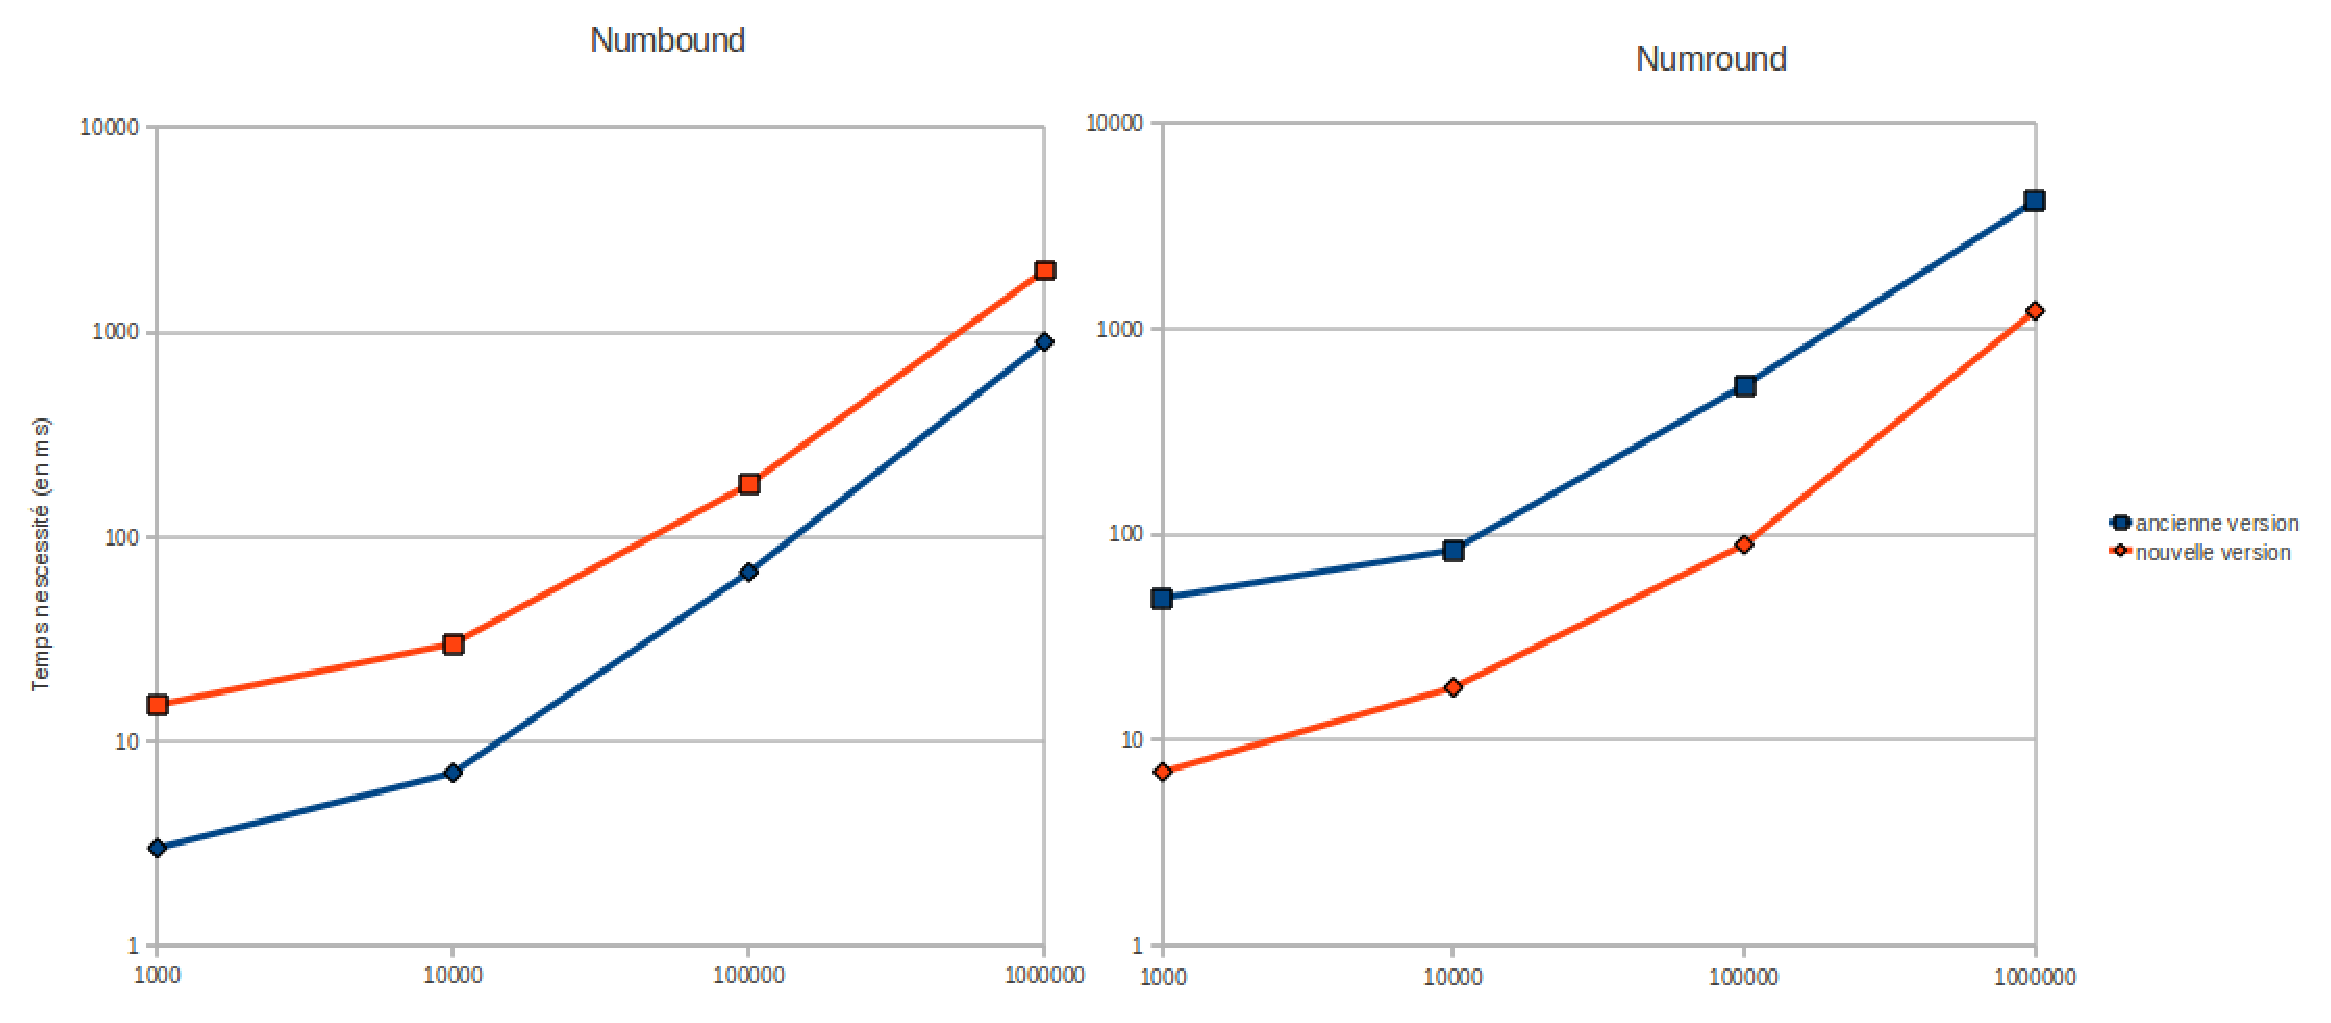
\includegraphics[width=10cm]{NumboundNumround.eps}
\end{center}
\caption{Performances de Numbound et Numround}
\end{figure}

\begin{table}[h]
\begin{center}
\begin{tabular}{|c|c|c|c|c|}
\hline
Nb de donn\'ees & numinterval (og) & numinterval (ng) & numnormalize (og) & numnomrmalize (ng)\\
\hline
 \multirow{2}*{100} & 2075 (fuites) & 101 & 1693 (fuites) & 6 \\
\cline{2-5}
 & 210ko & 40ko & 183ko & 16ko \\
\hline
 \multirow{2}*{1000} & 2075 (fuites) & 1001 & 1693 (fuites) & 12 \\
\cline{2-5}
 & 210ko & 4Mo & 183ko & 262ko \\
\hline
 \multirow{2}*{10000} & 2075 (fuites) & 10000 & 1693 (fuites) & 16 \\
\cline{2-5}
 & 210ko & 400Mo & 183ko & 2Mo \\
\hline
 \multirow{2}*{100000} & 2075 (fuites) & 100000 & 1693 (fuites) & 19 \\
\cline{2-5}
 & 210ko & 40Go & 183ko & 16Mo \\
\hline
\end{tabular}
\caption{Utilisation de la m\'emoire de numinterval et de normalize (nombre d'allocations et m\'emoire allou\'ee}
\end{center}
\label{tab:numbound}
\end{table}

\begin{figure}[h]
\begin{center}
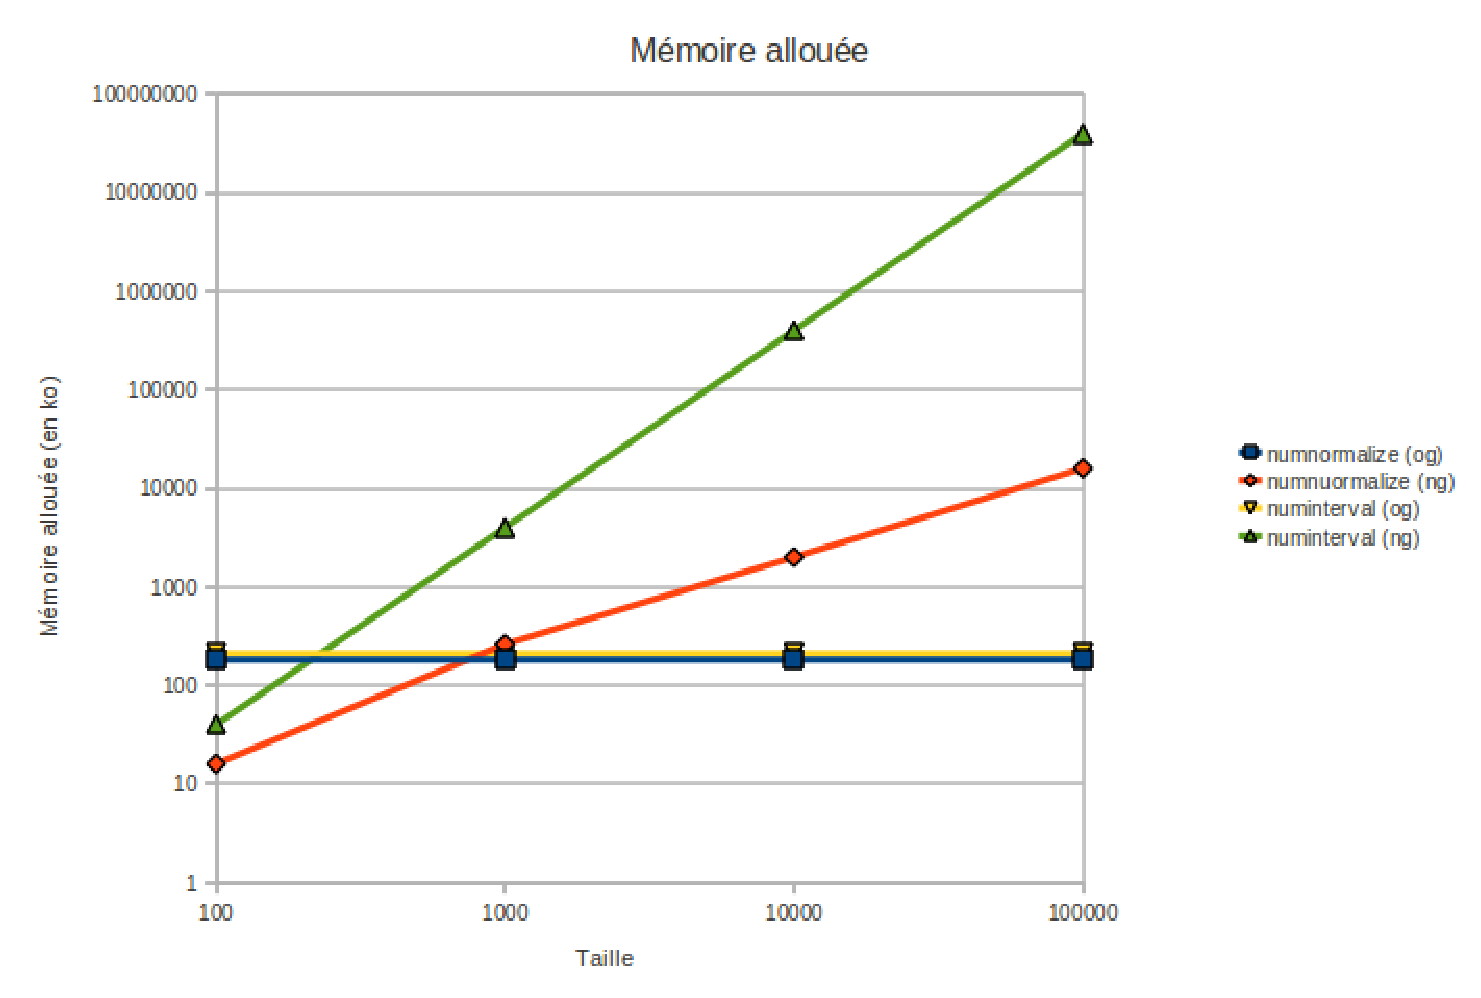
\includegraphics[width=9cm]{Memallouee.eps}
\end{center}
\caption{Utilisation de la m\'emoire pour numinterval et numnormalize}
\end{figure}

Les r\'esultats sont particuli\`erement exceptionels en mati\`ere de temps d'ex\'ecution mais il persiste le probl\`eme de l'utilisation de la
 m\'emoire pour numinterval.
\newline

\subsection{G\'en\'eration et modifications de nombre d\'ecimaux}

Dans cette partie la probl\`ematique est diff\'erente car aucun de ces programmes n'est destin\'e \`a travailler sur des flux de donn\'ees, 
d'ailleurs numrange et numrandom n'ont m\^eme pas de fichier en argument ils ne servent qu'\`a g\'en\'erer des nombres ou s\'eries de nombres.
C'est pourquoi on effectue differents tests pour ces fonctions : pour numgrep et numprocess on peut toujours regarder leur comportement selon la taille du fichier d'entr\'ee.
Tandis que pour numrange on peut faire augmenter la taille du fichier \`a g\'en\'erer et pour numrandom la taille de l'interval dans lequel on prend le chiffre.
Pour numprocess nous avons fait les tests pour plusieurs op\'erations et expressions seules certaines ont \'et\'e retenues pour le rapport.
Les tableaux de performance se trouvent en annexe.

\begin{figure}[h]
\begin{center}
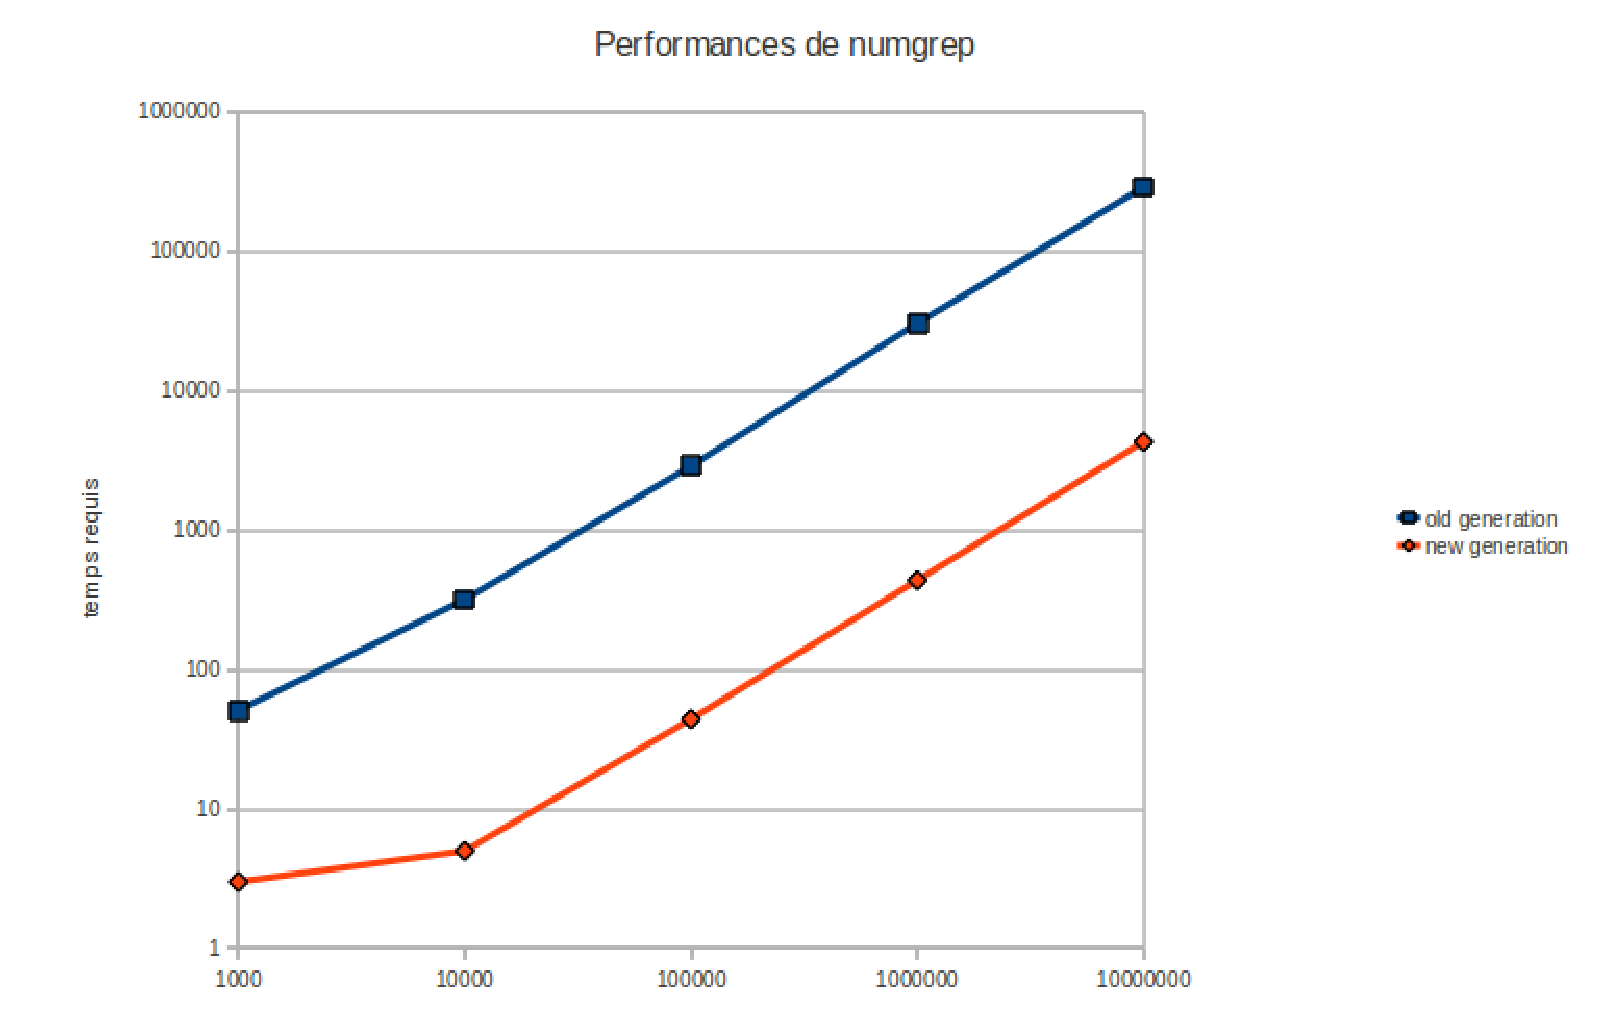
\includegraphics[width=9cm]{numgrep.eps}
\end{center}
\caption{Performances de numgrep}
\end{figure}

\begin{figure}[h]
\begin{center}
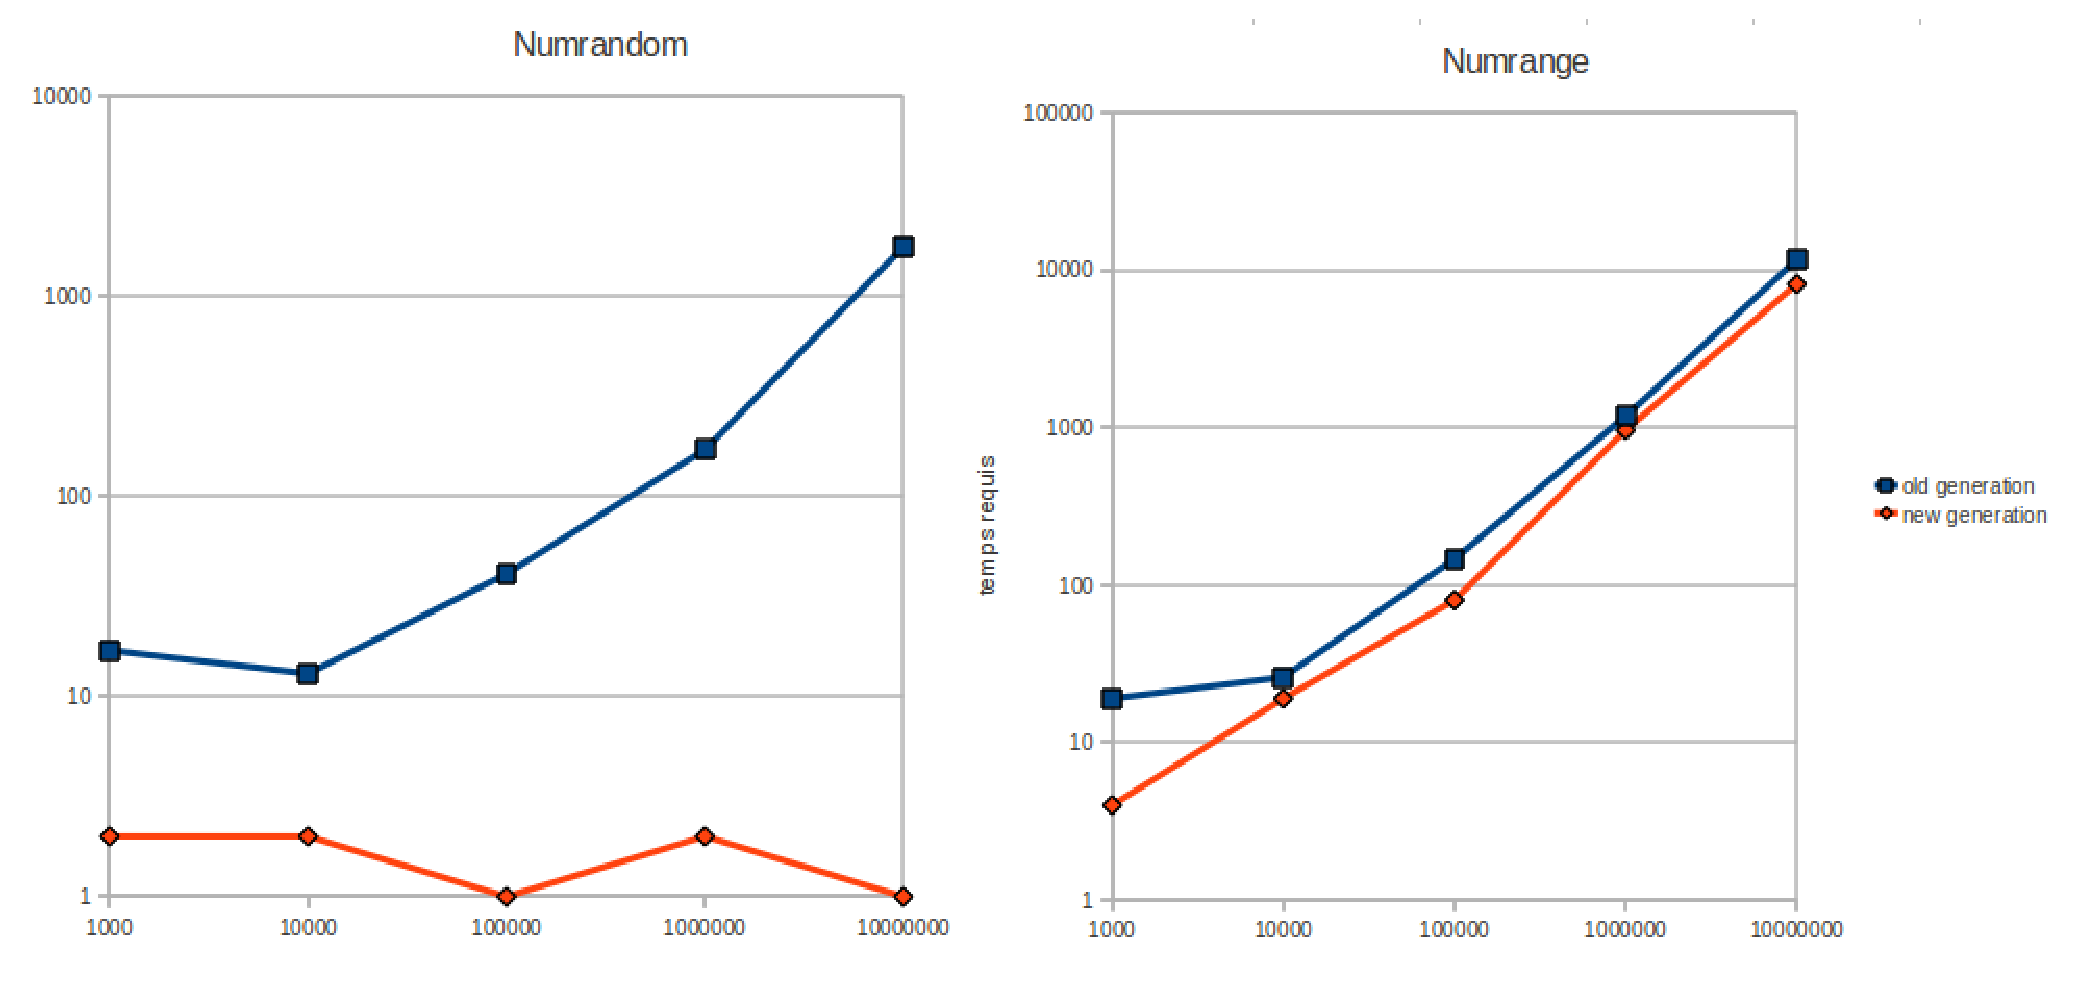
\includegraphics[width=15cm]{randomrange.eps}
\end{center}
\caption{Performances de numrandom et numrange}
\end{figure}

\begin{figure}[h]
\begin{center}
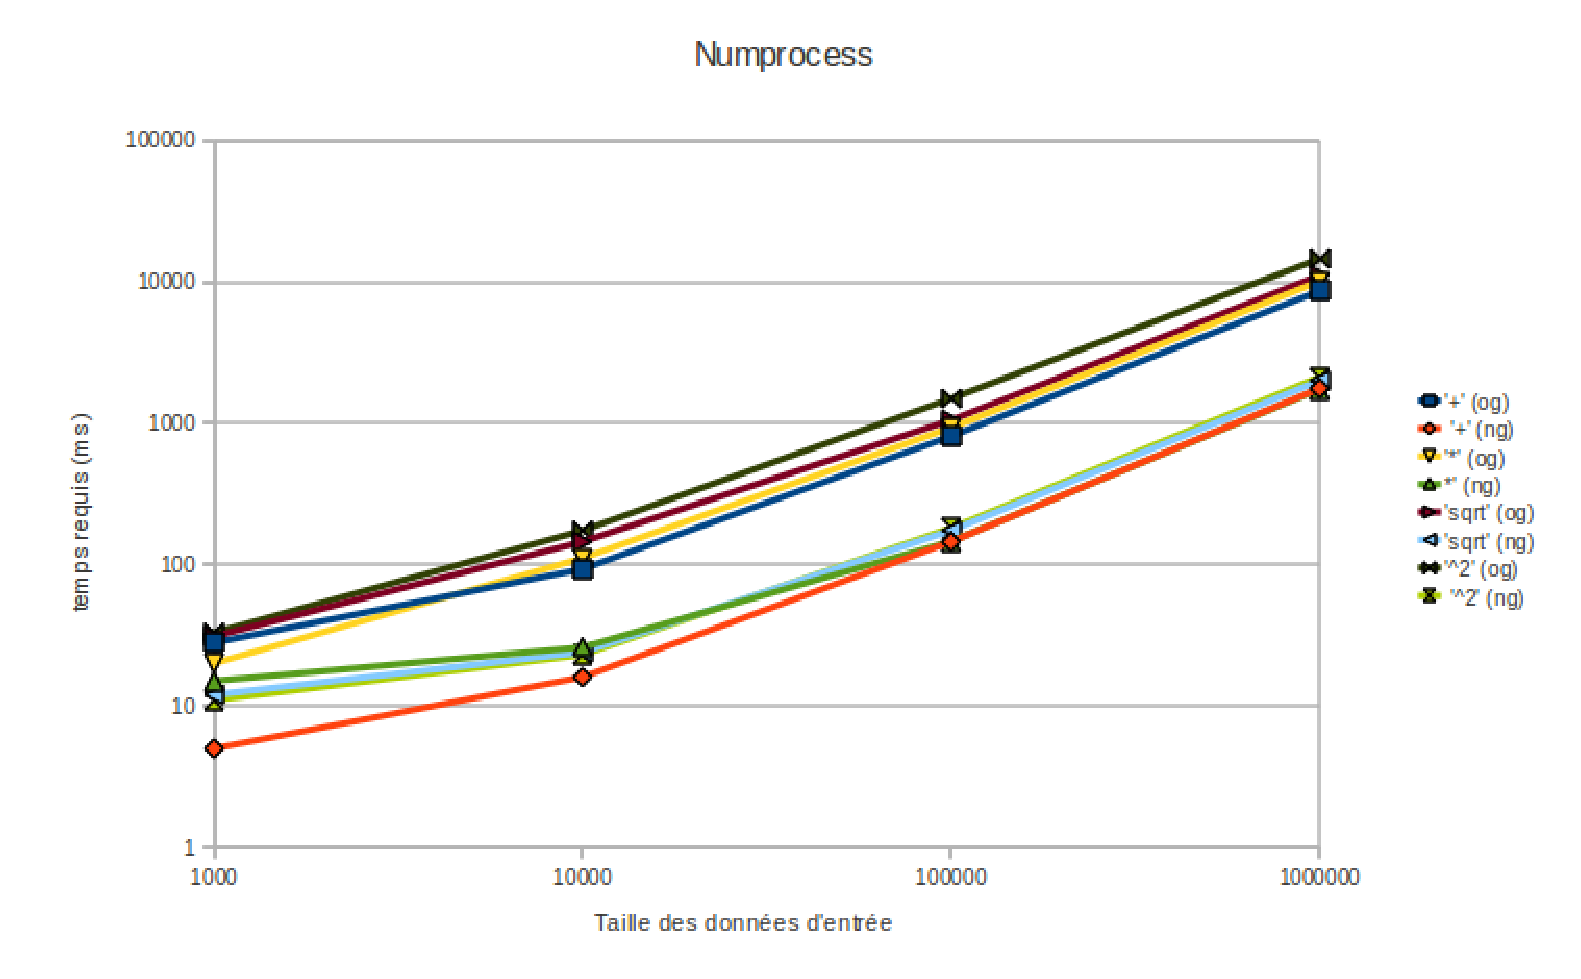
\includegraphics[width=9cm]{numprocess.eps}
\end{center}
\caption{Performances de certaines op\'erations de numprocess}
\end{figure}

Les r\'esultats en terme de temps pour numgrep et numprocess sont plut\^ot bons, il ny a quasiment pas d'utilisation de la m\'emoire dans numprocess et numrange contrairement aux anciennes versions. 
Nous avions aussi fait des tests en changeant le nombre d'intervalles dans les expressions et on peut voir que la progression est lin\'eaire, les programmes se comportent donc bien si il y a beaoup d'intervalles.

On peut ajouter que les programmes de l'ancienne biblioth\`eque comportent tous des fuites de m\'emoires (memory leaks) qui ne sont plus pr\'esent 
dans notre biblioth\`eque.

\section{Optimisation}

Nous avons vu les probl\`emes li\'es \`a la gestion des flux, il y a differents moyens pour pallier \`a ce probl\`eme, 
C'est ce que nous allons voir dans cette partie.

L'optimisation n'ayant pas \'et\'e termin\'ee cette partie n'est pas encore r\'edig\'ee